%%%%%%%%%%%%%%%%%%%%%%%%%%%%%%%%%%%%%%%%%%%%%%%%%%%%%%%%%%%%%%%%%%% 
%                                                                 %
%                            CHAPTER THREE                          %
%                                                                 %
%%%%%%%%%%%%%%%%%%%%%%%%%%%%%%%%%%%%%%%%%%%%%%%%%%%%%%%%%%%%%%%%%%% 
  
\chapter{Methods} \label{sec:methods}

In this chapter, we detail the finalized algorithm pipeline, as well as some alternative approaches that we found to have limited successs.

\section{Trailing Edge Extraction}

Extracting good, high quality trailing edges images is one of the primary challenges when matching Humpback whales by their trailing edge.
In this section, we describe the steps that go into automating the extraction of high quality trailing edges, while trying to minimize human intervention.

One major assumption we make when extracting these trailing edges is that the humpback whale fluke is aligned such that its major axis is horizontal.
Additionally, we generally assume that all parts of the fluke are present, however theoretically it would be possible to match a partial fluke -- although unlikely.

While these assumptions do not make for an incredibly robust system, the nature of the problem (and the dataset that we had at hand) makes these assumptions reasonable.
It would also be possible to add a detection step beforehand to ensure this assumption, however we do not explore this in this work.

\subsection{Fluke keypoint prediction}


\begin{figure*}[t]%
\centering
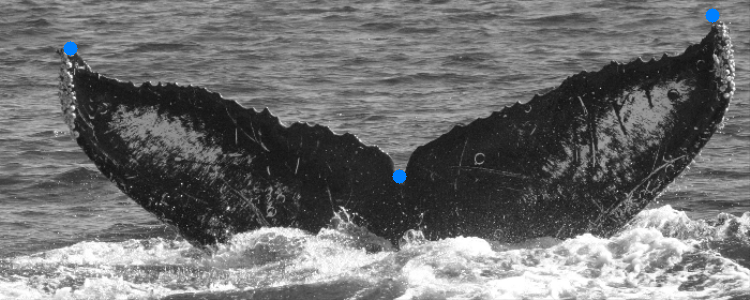
\includegraphics[width=1.0\textwidth]{../images/aid88_kpoverlay.png}
\caption[]{\textbf{Example Keypoint Prediction}. Example image showing the left tip, bottom of the notch, and right tip located by the keypoint extractor convolutional network.}
\label{fig:example_kp}
\end{figure*}


One major issue with automating the above trailing edge extraction algorithm is that it requires manual annotation in the selection of the starting and ending points (i.e., the fluke keypoints), as well as any control points (specifically the bottom of the notch).
To work around this, we propose a convolutional network that predicts these tip points as part of the identification pipeline.

When extracting trailing edges, one of the first steps we take is to identify the starting and ending points of the trailing edge, as well as the bottom of the central notch.
To do this, we train a convolutional network to predict these three points.

The convolutional network does not need full-sized images, so the first step of the keypoint extraction pipeline is to resize the image to $256 \times 256$ pixels.
This size choice is somewhat arbitrary, but we find that it provides the best performance without using an unnecessary amount of memory.
The network then predicts the points as values between $0$ and $1$, for both the width and height of the image. 
These predictions are then then rescaled back up to the original image size.
An example prediction is shown in Figure \ref{fig:example_kp}.
%The evaluated network architectures are detailed in Table 3.1. % TODO put this in

\subsubsection{Network Design}

The overall design of the network follows the pattern of alternating small ($3 \times 3$) convolutional filters with $2 \times 2$ max pooling layers, at each step doubling the number of channels (starting with $8$ channels).
This is somewhat similar to VGG-16, although with half the trainable layers.
After a $32\times$ downsample has been achieved, we attach a decision layer which consists of a dense layer followed by three separate dense layers with separate predictions layers after (one for each point being predicted).
While this is not a common approach in keypoint prediction, we found that it gave better performance than having the points predicted as a single vector.

We theorize that this may be because shared units between each of the three predictions leads to stronger correlations between them, reducing overall prediction flexibility.

\subsubsection{Training Details}

Generating the training data for this is straightforward given a set of annotations with the associated points to learn.
The dataset that we created for this purpose contains approximately $2100$ training images, $700$ validation images, and $900$ test images.

First, each image is resized to a fixed width while maintaining the aspect ratio.
This is done to somewhat normalize the relative scale of objects in each image on the assumption that they are constrained to contain the fluke.
Each image is rescaled to the network size, and then the corresponding targets are rescaled to the range $[0-1]$.
The size of the original image is recorded as well.
While it would be possible to treat this as a simple multi-variate regression and use RMSE loss, we achieved better results by averaging the Euclidean distance between the predicted points and true points.
We also include a scalar scaling factor $\alpha$, which scales each point by a proportion of the original image size.
Thus, we have the scaled Euclidean loss $SE$

\begin{equation} \label{eqn:se_loss}
SE(\vec{t}, \vec{p}, \vec{s}, \alpha) = \lVert (\alpha * \vec{s}) \odot (\vec{t} - \vec{p}) \rVert
\end{equation}
Where
\begin{itemize}
    \item $\vec{t}$ and $\vec{p}$ are the $(x, y)$ ground truth and predicted values respectively
    \item $\vec{s}$ is the original image width and height
\end{itemize}

The networks are trained for 1000 epochs with $\alpha$ set to \num{2e-2} using the Adam \cite{kingma2014adam} optimizer (with recommended settings) and $l2$ regularization on the trainable parameters with a decay of \num{1e-4}.
All of these hyper parameters were tuned using the validation set, although the possible parameter space was not fully explored due to time constraints.

\subsubsection{Evaluation} % TODO: Maybe this should be moved to the results section?

%TODO Put in a bunch of figures and talk about this
% Problem is recreating all these experiments / networks for evaluation :/
% Might take a while...

On average, the best network achieved a 10 pixel distance error on the validation and testing sets (in the original image scale).
While this may seem like a lot, the trailing edge extraction (and subsequent matching accuracy) was not severely affected when only using the start and end point predictions.

%Additionally, as can be seen in Figure 3.2, 
We find that, for the vast majority of images, the network achieves a low pixel distance error, while there are a few that have a much higher error.
Qualitative inspection of these images shows that they are either of flukes which are not the singular or major object in the image, or horizontally oriented of flukes that are not horizontally rotated.
An example of this is shown in Figure \ref{fig:example_kp}.

%  TODO: Figure showing this

\begin{figure*}[t]%
\centering
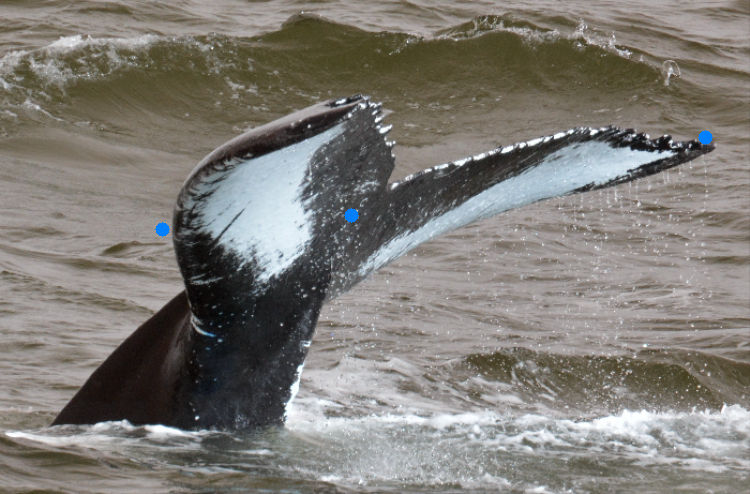
\includegraphics[width=1.0\textwidth]{../images/aid1323_kpoverlay.png}
\caption[]{\textbf{Example Keypoint Failure}. Example image showing a keypoint extraction failure case from its testing set. Note the difference in pose of the fluke from the success case shown in Figure \ref{fig:example_kp}}
\label{fig:example_kp_failure}
\end{figure*}



We attempted to use a spatial transformer network \cite{jaderberg2015spatial} to try and handle these cases, but we were unable to get it to perform as well as the standard convolutional network, nor produce sensible transformations.
Since these failure cases represent a small amount of the dataset

\subsection{Basic Trailing Edge Extraction Algorithm}

% TODO: Picture of I_y

The base algorithm that is used for extracting the trailing edge uses the vertical gradient information of the image (denoted as $I_y$).
We extract $I_y$ using a vertically oriented $5 \times 5$ Sobel kernel \cite{Sobel1968}.  

We then normalize $I_y$ with min-max scaling, giving $N_y$ as

\begin{equation} \label{eqn:norm01}
N_{y} = \frac{I_y - \min(I_y)}{\max(I_y) - \min(I_y)}
\end{equation}

With $N_y$, we then need a starting point and ending point for the algorithm, denoted $s$ and $e$ respectively, with their $x$ and $y$ coordinates being denoted with subscripts. 

For our purposes, we use the left and right tips of the fluke as our start and end points respectively.
Additionally, we experiment with using the bottom of the notch to aid the trailing edge extractor.
We explain how these points are determined in the next section.

Given a point $p$, we then set its corresponding column in $N_y$ to $\infty$, and set the point itself set to $0$. 

\begin{align} \label{eqn:te_setup}
N_y(p_x,\cdot) = \infty \\
N_y(p_x,p_y) = 0
\end{align}

This forces the path to ``go through'' these points. 
We do this for the start (i.e.\ left tip) and end points, as well as the bottom of the notch. 

The minimal path is then found by scanning the columns of $N_y$ from left to right, starting and ending at $s$ and $e$ respectively. 
For each pixel in a column we set its cost with the following update rule:

\begin{equation} \label{eqn:te_update}
C(x,y) = 
\begin{cases}
	0 & x < 0 \\
	\infty & y < 0 \text{ or } y > h \\
	\min_{y - n \leq y_c \leq y + n}(C(x-1, y_c) + N_y(x,y)) & \text{else} \\
\end{cases}
\end{equation}

Where $n$ is a neighborhood constraint and $h$ is the height of $N_y$.  
We default $n$ to $1$, meaning that each pixel considers $3$ 'neighbors' in the previous column.

As $C$ is filled out, we also keep a backtrace matrix $B$, which keeps track of the index of the minimal candidate chosen in equation \ref{eqn:te_update}.
Once the end column is reached, we work backwards from $e$ to construct the path, adding the coordinate corresponding to $B(x,y)$ at each step.

% Maybe: Put in actual algorithm pseudocode
% TODO: Put in pictures of extracted fluke, cost matrix?

We can also extend this algorithm by adding extra 'control points' which the path is forced through, using the same methodology as forcing the path through the start and end points.
Commonly, we use the bottom of the notch as a control point, although this affects accuracy negatively if it too far from the trailing edge.

While this algorithm has no understanding of humpback whale flukes, a lot of images that are constrained around the fluke with oceanic backgrounds (which is a large majority of the dataset at hand) provide high quality trailing edges when put through this algorithm.
However this is not a robust algorithm for finding trailing edges, something that we will fix later on.

% TODO: Put in figure showing bad trailing edge from raw next to good one

\subsection{Trailing Edge Scoring}

As mentioned in the beginning of this section, using only the gradient information for extracting the trailing edge works in a lot of cases, but is not a robust method.

If we had a score of each pixel's ``trailing edginess'' in an image, the trailing edge extractor could make use of this information to make better choices in trailing edge extraction.
To do this, we need a prediction of whether or not each pixel belongs to the trailing edge of a fluke, a task that is best suited to a fully convolutional network.
In these networks, all convolutions (aside from max pooling layers) are ``same'' convolutions, which have square, odd filters (usually $3 \times 3$) and 1-padding. % TODO: Maybe find a citation describing these?
These ``same'' convolutions produce a spatial output shape that is the same as the input shape, obviating the need for any interpolation.

The four major variants on trailing edge scoring networks that we evaluated are detailed below.
All of these networks function on the same paradigm of taking an arbitrarily sized image and producing an image of the same size but with a class score for each pixel.

The dataset was sourced from trailing edges extracted using the basic method detailed above, however with manual adjustments to fix many of the more common issues we encountered with this algorithm.

To generate the training set, we extract a $128 \times 128$ patch at $128$ pixel intervals along the trailing edge (giving a positive patch), and a corresponding patch (with no trailing edge pixels) randomly sampled from the left over space above and below the trailing edge (giving a negative patch).
These patches are then randomly split into training, testing, and validation sets each with $3700$, $1200$, and $1600$ patches respectively.

\subsubsection{Trailing Edge Scoring Architectures}

There are several network architectures that were tried, however here we will report only the major variants.
One major consideration that has to be made when selecting a fully convolutional network architecture is its receptive field.
If the receptive field is too small, it may not have enough information to accurately determine if a given pixel is part of the trailing edge.
However, in order to increase the receptive field without massively increasing the depth of a network, we must downsample, which makes the output less fine-grained.

\paragraph{Simple}
This network is simply a stack of $6$ "same" convolutional layers (of decreasing spatial extent), with no downsampling regions.
This has a small receptive field, but can produce detailed predictions.
Due to the small receptive field however, at convergence it gives low precision predictions, and seems to (in many cases) produce a lot of the same mistakes that normal gradient based trailing edges do.

\paragraph{Upsample}
To deal with the small receptive fields, convolutional networks typically downsample at various stages. 
This downsampling usually takes the form of max pooling (instead of e.g. convolutional kernels with a stride greater than one).
The upsample architecture is analogous to the FCN-32s architecture in \cite{long2015fully}, although we do not go down to a 1x1 spatial extent before upsampling.
This produces blocky and nearly unusable trailing edge scores, however they tend to be more connected than the disparate (but fine-grained) predictions made by the simple network.


\paragraph{Jet}
Following the deep-jet architecture from \cite{long2015fully}, we combine softmax predictions from various stages throughout the network with predictions from "farther down" the network, cascading until we hit predictions from the last convolutional layer before any downsampling.
This gives more fine-grained predictions than the upsample network while giving somewhat better predictions than the simple network.


\paragraph{Residual}
While the receptive field of the Simple network is small, it can produce very fine trailing edges, which we found to be necessary for good trailing edge extraction.
However with such a small receptive field it can be more prone to making mistakes.
It is possible to create a very deep network of 'same' convolutions, however training very deep networks like this can run into problems very quickly.
Recently, there has been work on making very deep networks feasible by adding residual connections\cite{he2015deep}, showing that these very deep networks can achieve high accuracy in a challenging benchmark.
We replicate this architecture by stacking $64$ $3\times3$ 'same' convolution kernels, and adding a residual connection every other layer.
This performs better than the Simple network, however we do not see a marked improvement in trailing edge matching as a result.

% TODO: Include images showing extracted trailing edge scores for all of these networks

\subsubsection{Using the trailing edge scores}

Once we have 'trailing edginess' score for each pixel, we need to combine this information with the gradient in a way that causes the trailing edge extraction algorithm to follow those pixels that the scoring map marks as trailing edge.
More formally, the trailing edge scoring map gives us an image $T_p \in [0-1]^{w \times h}$ (where $w$ and $h$ are the width and height of the image) which denotes the network's predicted probability of each pixel being part of the trailing edge.
The most simple and obvious way to combine this information with $N_y$ from before is to combine them with a mixing parameter $\beta$.

\begin{equation}
S_{te} = (1 - \beta)*N_y + \beta*(1 - T_p)
\end{equation}

We use $1 - T_p$ in this case because we are minimizing the path through $S_{te}$.
Once done, the trailing edge extraction algorithm procedes as described in the previous section.

For most of the evaluation process, we simply set $\beta = 0.5$.

Another variant on combining $T_p$ and $N_y$ that we tried was to dilate the trailing edge predictions and then forbid the trailing edge from going outside of those predictions.
However one of the main issues with this is that if there are any breaks in the prediction (which can happen even with the Upsample architecture), the trailing edge cannot be extracted, leading to broken trailing edges.

\subsubsection{Training Details}

All networks were trained for 100 epochs (or until convergence) with a batch size of $32$, with $l2$ regularization using a decay of \num{1e-4}.
We used the Adam optimizer\cite{kingma2014adam} (with the recommended settings) for calculating weight updates.

One detail that turned out to be important is the class imbalance.
The trailing edge pixels (necessarily) make up a small percentage of the total image, meaning that these networks could get a fairly high accuracy (and thus low loss) simply by predicting only background pixels.
In order to prevent this, we only sample a negative patch once for every positive patch (as detailed above), and additionally we weight the loss for the trailing edge pixels $10\times$ higher than the loss for the background pixels.

Due to the nature of the training data, we were concerned that the networks would simply learn to replicate the function that generated the trailing edges, despite human corrections.
In order to mitigate this issue, we included some non-spatial data augmentation, namely random Gaussian blur and randomly inverting the pixel intensities.
Unfortunately this had limited success.

% TODO: Show failures

All of these hyper parameters were tuned using the validation set, although the possible parameter space was not fully explored due to time constraints.

\subsubsection{Evaluation}

Due to the overwhelming class imbalance, the model accuracy is rather meaningless (e.g.\ the accuracy of an all-background prediction is $99\%$).
Instead, we report the intersection-over-union (IoU) score, which gives a much better idea of model performance.
We also report the precision and recall of the model.

% IOU / PRECISION / RECALL
% TRAIN / TEST / VAL
% SIMPLE / UPSAMPLE / JET / RES


\begin{table*}[!htb]%
	\centering
	\resizebox{\linewidth}{!}
	{
		\begin{tabular} {l || l | l | l || l | l | l || l | l | l |}
		& \multicolumn{3}{c||}{Training} & \multicolumn{3}{c||}{Validation} & \multicolumn{3}{c|}{Testing} \\
		\hline
		Architecture & Pr. & Re. & IoU & Pr. & Re. & IoU & Pr. & Re. & IoU \\
		\hhline{=#===#===#===|}
		Simple & 0.59 & 0.95 & 0.57 & 0.59 & 0.94 & 0.57 & 0.60 & 0.95 & 0.59 \\
		\hline
		Upsample & 0.17 & 0.88 & 0.17 & 0.17 & 0.86 & 0.17 & 0.17 & 0.87 & 0.17 \\
		\hline
		Jet & 0.62 & 0.89 & 0.57 & 0.62 & 0.88 & 0.57 & 0.63 & 0.89 & 0.58 \\
		\hline
		Residual & 0.57 & 0.93 & 0.54 & 0.57 & 0.92 & 0.54 & 0.58 & 0.93 & 0.56 \\
		\hline
		\end{tabular}
	}
	\caption{Table showing the precision, recall, and IoU of each of the evaluated trailing edge scorers on each section of the trailing edge dataset. For the purposes of this analysis, we use the \texttt{argmax} over the classes to determine a positive (i.e. trailing edge) or negative pixel.}
	\label{tab:te_score_full_analysis}
\end{table*}

Initially, we thought that precision would be the most important metric for evaluating networks (which is reflected in the class weighting).
However, we found that even a low precision classifier could give good trailing edges, and that the important measure was how detailed these trailing edges were.

% TODO: Figure showing this

This is likely because small segments of predicted trailing edge would not be chosen by the trailing edge extractor if they are too disconnected from the actual trailing edge.

\section{Trailing Edge Matching}

Given extracted trailing edges, we define a method for doing a one-to-one comparison between a given query and database trailing edge.
%Once these trailing edges are extracted, we can use a few simple methods to compare them in search of a trailing edge that is close to the one we are finding a match for.
The simplest way to do this is to define a (potentially non-metric) distance function between any two trailing edges.
Once this distance function is defined, we can identify an individual by its trailing edge (referred to as the query trailing edge) by looking at the identity of the closest trailing edge in the database.
As a distance function we use dynamic time warping over block curvature measurements, using a weighted Euclidean distance as a local distance function between curvatures.

\subsection{Curvature Measurement}

In order to do this, we must first extract the curvature from the trailing edge.
Given the trailing edge as a sequence of coordinates into the original image, we construct a zero-image $I_0$ of shape similar to the original image.
Each pixel corresponding to and below the trailing edge in $I_0$ is set to $1$.
Because the trailing edge extractor produces only one coordinate per column, we can do this safely, however this algorithm could be easily adapted to this not being the case.
Once this is done, we calculate a summed area table \cite{crow1984summed} $ST$ from $I_0$ as follows.

\begin{equation} \label{eqn:sat}
ST(x,y) = \sum_{i=0}^{i=y}\sum_{j=0}^{j=x} I_0 
\end{equation}

Conceptually, the next step is to slide a square of shape $s \times s$ centered on each point, and measure the percentage of that square that is within the filled in trailing edge.
These values $s$ are the different scales at which we meassure curvature, and are computed as a percentage of the trailing edge length.

To do this, we compute $BC_s(x, y)$ for each $(x, y)$ coordinate in the trailing edge.

\begin{align} \label{eqn:sat_area}
\begin{split}
b(i) &= i - \frac{s}{2}\\
e(i) &= i + \frac{s}{2}\\
BC_s(x,y) &= \frac{(ST(b(x), b(y)) + ST(e(x), e(y))) - (ST(b(x), e(y)) + ST(e(x), b(y)))}{s^2}
\end{split}
\end{align}

The numerator in equation \eqref{eqn:sat_area} gives the total area within the square that is below the trailing edge, which we then normalize by dividing by the square's area.

The set of scales to choose presents a large parameter space, however we have found that the scales $S = [2\%, 4\%, 6\%, 8\%]$ work well for our purposes.
We then treat this curvature measurement as a $|S| \times l$ matrix $BC$, where $l$ is the length of the trailing edge.

\subsection{Sequence Matching}

Given two sequences of curvatures $BC_1$ and $BC_2$ (referred to as query and database curvature respectively) we match them using dynamic time warping as follows.
First, we create a cost matrix $C$ of size $l_1 \times l_2$. 
We initialize this cost matrix by setting the first column and row to $\infty$, and then $C(0,0) = 0$, intuitively forcing the optimal path to match align the beginning of $BC_1$ with $BC_2$.
Then, for each cell $(i,j)$ in the cost matrix starting with $C(1,1)$, we use the following update rule

\begin{align} 
\label{eqn:dtw_dist}
D_{\vec{s_w}}(c_1, c_2) &= \lVert \vec{s_w} \odot (\vec{c_1} - \vec{c_2}) \rVert_2\\
\label{eqn:dtw_update}
C(i,j) &= D_{s_w}(BC_1(i,\cdot),BC_2(j,\cdot)) + min(C(i-1,j), C(i,j-1), C(i-1, j-1))
\end{align}

Where $\vec{s_w}$ is a vector giving the weight for each curvature scale, and $\vec{c}$ is a vector of the curvatures at different scales for a point.

Additionally, we impose the Sakoe-Chiba \cite{sakoe1978dynamic} locality constraint $T$ so that for each element $i$ in $BC_1$, we only consider the range over elements $j$ in $BC_2$ of $j \in [min(i - T, 0), max(i + T, l_2)]$.

We set $T$ as a percentage of $l_1$.
For most of these experiments $T$ is set to $10\%$, which appears to minimize the time taken for each comparison while preserving the overall accuracy of the algorithm.

It's worth noting that while this distance measure is not a metric distance (i.e.\ it doesn't satisfy the triangle inequality), it is a symmetric distance as \eqref{eqn:dtw_dist} is symmetric \cite{muller2007information}.

\section{Alternative Approaches}

In this section, we list and briefly describe alternative approaches that were tried, although they did not prove accurate enough to make it into the final system.

\subsection{Aligning Trailing Edges}

One obvious pre-processing step that would make sense when comparing trailing edges is to make sure that they are aligned in image space.
However, we found that doing so when comparing curvature was often unnecessary (due to the invariances to rotation and translation, scale was taken care of separately), and using the Euclidean distance between points on the aligned trailing edges (i.e.\ in place of curvature for \eqref{eqn:dtw_dist}) did not give good results.

There were two approaches to alignment that we evaluated, although neither achieved top-1 accuracies above $20\%$.

\subsubsection{Keypoint Alignment}

As noted in the section on fluke keypoints, there are three points to predict --- left, notch and right.
Originally the intention for recording (and predicting) all three, as opposed to just left and right, was to have three corresponding points with which to estimate an affine transformation from database image onto query image.
This would be done prior to any computation of trailing edge or curvature.

One major issue with aligning these iamges however is that if a non-affine transformation was required, the trailing edge itself would be warped in such a way that made matching difficult.

\subsubsection{Dynamic Time Warping Alignment}

Taking after the AI-DTW approach laid out in \cite{qiao2006affine}, we ran an iterative alignment process that used the correspondences found by DTW (using either curvature distance or Euclidean distance as criteria).
Essentially this method would find alignments using DTW, and then use these alignments to estimate an affine transformation of the database image onto the query image -- and then repeat until convergence.

However, we found that this process oftentimes wouldn't converge, and when it did the alignments provided were of worse quality than those found by aligning the three fluke keypoints.
Additionally, the extra time taken to carry out this process was impractical.

\subsection{Histogram Matching}

One early curvature comparison method that we evaluated was to use histograms to match instead of a sequence-based method.
This is a common approach for comparing curvatures \cite{kumar2012leafsnap}, however we found that for our purposes even high resolution histograms did not provide enough detail to match the trailing edges properly, although this could potentially be explored further.

\subsection{Embedding via Convolutional Networks}

We also made an attempt at training convolutional networks to directly embed the images of flukes into a $n$ dimensional vector, much like \cite{schroff2015facenet} and \cite{parkhi2015deep}.
However, most of the previous literature on this technique is applied to larger datasets such as LFW\cite{huang2007labeled}, which is significantly larger than the dataset that we had available.
A major factor in this is that these larger datasets often have five to ten images per identity (if not more), whereas most of the identities in our dataset had one or two images associated.

Regardless, we attempted the embedding approach (from raw images), however even a severely overfit convolutional network only achieved half the top-1 accuracy on its training set that the main method is able to achieve.
We tried both triplet loss (a modified version of the one detailed in \cite{schroff2015facenet}) and contrastive loss \cite{hadsell2006dimensionality} to no avail.

We believe that the small amount of images per identity is the main factor for the failure of these methods, and that a larger dataset would be necessary to properly train them.

%%% Local Variables: 
%%% mode: latex
%%% TeX-master: t
%%% End: 
